\begin{figure}[htb]
    \centering
    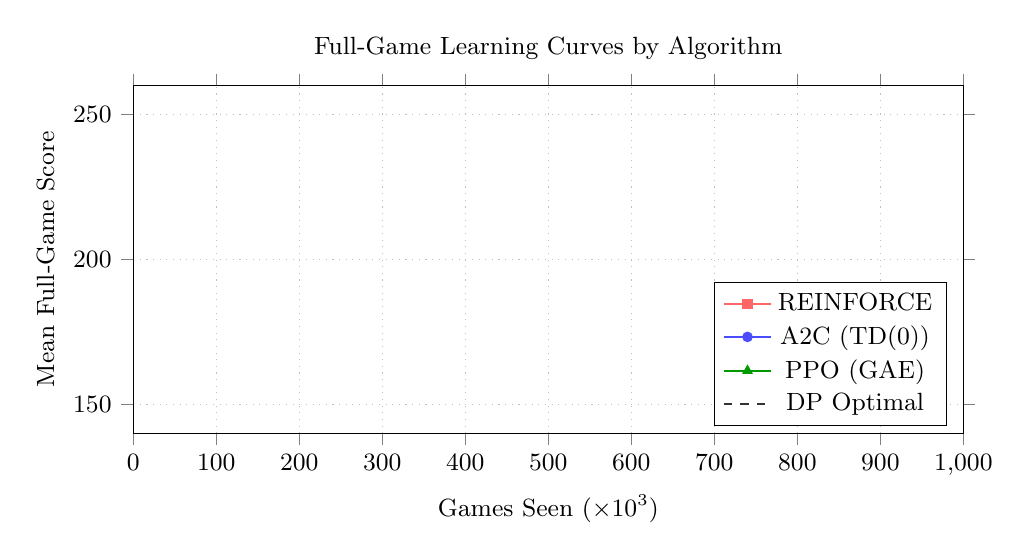
\begin{tikzpicture}
        \begin{axis}[
                width=\columnwidth,
                height=6cm,
                xlabel={Games Seen ($\times 10^3$)},
                ylabel={Mean Full-Game Score},
                title={Full-Game Learning Curves by Algorithm},
                xmin=0, xmax=1000,
                ymin=140, ymax=260,
                grid=both,
                grid style={dotted},
                tick align=outside,
                tick label style={font=\small},
                label style={font=\small},
                title style={font=\small},
                legend style={at={(0.98,0.02)},anchor=south east,font=\small}
            ]

            % REINFORCE learning curve
            \addplot[
                thick,
                red!60!white,
                mark=square*,
                mark size=1.5pt,
                mark repeat=20
            ] coordinates {
                    (0, 50)
                    (100, 50)
                    (200, 50)
                    (300, 50)
                    (400, 50)
                    (500, 50)
                    (600, 50)
                    (700, 50)
                    (800, 50)
                    (900, 50)
                    (1000, 50)
                };
            \addlegendentry{REINFORCE}

            % A2C learning curve
            \addplot[
                thick,
                blue!70!white,
                mark=*,
                mark size=1.5pt,
                mark repeat=20
            ] coordinates {
                    (0, 50)
                    (100, 50)
                    (200, 50)
                    (300, 50)
                    (400, 50)
                    (500, 50)
                    (600, 50)
                    (700, 50)
                    (800, 50)
                    (900, 50)
                    (1000, 50)
                };
            \addlegendentry{A2C (TD(0))}

            % PPO learning curve
            \addplot[
                thick,
                green!60!black,
                mark=triangle*,
                mark size=1.5pt,
                mark repeat=20
            ] coordinates {
                    (0, 50)
                    (100, 50)
                    (200, 50)
                    (300, 50)
                    (400, 50)
                    (500, 50)
                    (600, 50)
                    (700, 50)
                    (800, 50)
                    (900, 50)
                    (1000, 50)
                };
            \addlegendentry{PPO (GAE)}

            % DP optimal baseline
            \addplot[
                dashed,
                black!80,
                thick,
                domain=0:1000
            ] {50};
            \addlegendentry{DP Optimal}

        \end{axis}
    \end{tikzpicture}
    \caption{Algorithm comparison learning curves (placeholder data)}
    \label{fig:full-game-learning-curves}
\end{figure}